\chapter{État de l'art}

\section{RESTful}

REST(REpresentational State Transfer) \cite{Fie00} est un principe d'architecture qui s'applique aux services Web. Il ignore les détails de l'implémentation des composants et de la syntaxe de protocole afin de se concentrer sur les rôles des composants, les contraintes liées à leurs interactions avec d'autres composants et leurs interprétations des éléments de données significatifs. Il englobe les contraintes fondamentales sur les composants, les connecteurs et les données qui définissent la base de l'architecture Web. Le serveur et le client communiquent sans que le client ne connaisse les informations stockées sur le serveur.
\newline

\noindent
En architecture REST, on utilise des requêtes HTTP pour interagir entre le client et le serveur :
\begin{itemize}
    \item Créer (create) $\Rightarrow$ POST
    \item Afficher (read) $\Rightarrow$ GET
    \item Mettre à jour (update) $\Rightarrow$ PUT
    \item Supprimer (delete) $\Rightarrow$ DELETE
\end{itemize}

\noindent
L'architecture REST est régie par des contraintes :

\begin{itemize}

    \item \textbf{Client / Serveur} :
    \newline
    Il faut séparer les problèmes d’interface utilisateur des problèmes de stockage de données, cela permet d'améliorer la portabilité de l'interface utilisateur sur plusieurs plates-formes ainsi que l’évolutivité en simplifiant les composants du serveur.

    \item \textbf{Stateless} :
    \newline
    La communication doit être sans état, chaque demande du client au serveur doit contenir toutes les informations nécessaires pour comprendre la demande et ne peut tirer parti d'aucun contexte stocké sur le serveur. L'état de la session est donc entièrement conservé sur le client. Cela permet d'induire des propriétés de visibilité, de fiabilité et d'évolutivité.

    \item \textbf{Cache} :
    \newline
    Les contraintes de cache exigent que les données contenues dans une réponse à une demande soient étiquetées de manière implicite ou explicite comme pouvant être mises en cache ou non. Si une réponse peut être mise en mémoire cache, un cache client reçoit le droit de réutiliser ces données de réponse pour des demandes équivalentes ultérieures.

    \item \textbf{Interface uniforme} :
    \newline
    La caractéristique centrale qui distingue le style architectural REST est l'accent mis sur une interface uniforme entre les composants. Cela permet à l'architecture globale du système d'être simplifiée et la visibilité des interactions d'être améliorée.

    \item \textbf{Système en couches} :
    \newline
    Le système en couches permet à une architecture d'être composée de couches hiérarchiques contraignante, cela implique que chaque composant ne peut échanger qu'avec la couche immédiate. Cela permet de limiter la complexité du système. Les couches peuvent être utilisées pour encapsuler des services existants et protéger les nouveaux services des clients existants. Les intermédiaires peuvent également être utilisés pour améliorer l'évolutivité du système en permettant l'équilibrage de la charge des services sur plusieurs réseaux et processeurs.

    \item \textbf{Code à la demande} (Facultatif):
    \newline
    Le principe du code à la demande est de pouvoir étendre les fonctionnalités du client en téléchargeant et en exécutant du code sous la forme d'applets ou de scripts. Cela simplifie les clients en réduisant le nombre de fonctionnalités devant être pré-implémentées et permet d'ajouter de nouvelles fonctionnalités ultérieurement.

\end{itemize}

\section{Schéma des méthodes RTBH}

Dans cette section, nous vous présentons les schémas explicatifs des méthodes RTBH expliqué dans l'\hyperref[sec:intro]{introduction}.

\newpage

\subsection{Destination-based Black hole}

\begin{figure}[H]
    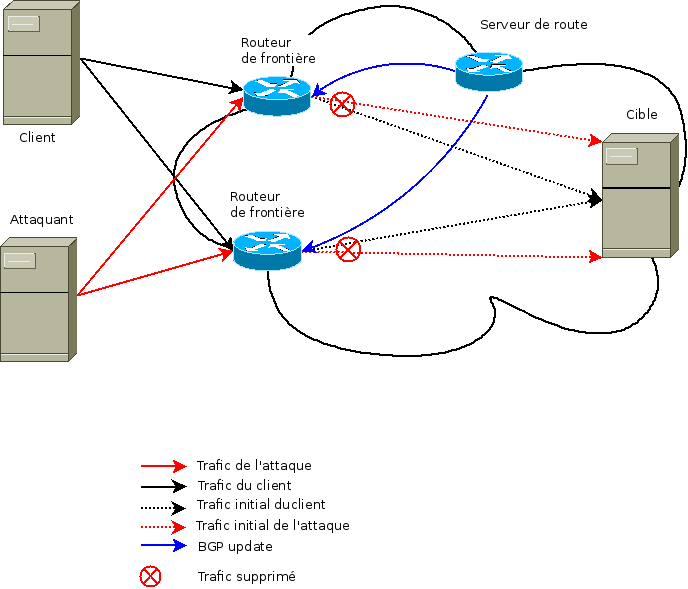
\includegraphics[width=\textwidth]{schema_destination_based.png}
    \caption{Destination-based black hole}
    \label{fig:destination_based}
\end{figure}

Comme on peut le voir, cette contre-mesure pose des problèmes car le client ne peut plus accéder au serveur. L'attaquant a donc réussi son objectif.

\subsection{Source-based Black hole}

\begin{figure}[H]
    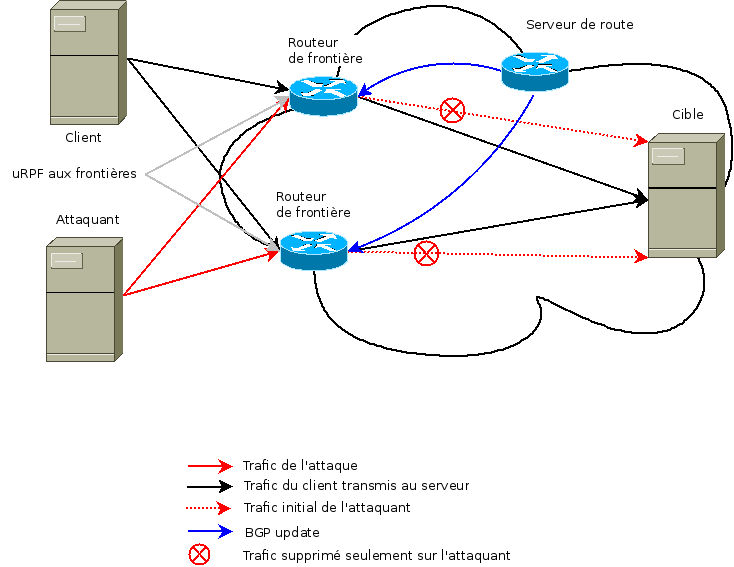
\includegraphics[width=\textwidth]{schema_source_based.png}
    \caption{Source-based Black hole}
    \label{fig:source_based}
\end{figure}

Grâce à cette méthode, le client peut toujours communiquer avec le serveur alors qu'avec la méthode précédent ce n'est pas le cas.

\section{BGP}
\label{sec:BGP}

Le protocole BGP \cite{Rfcbgp06}, Border Gateway Protocol, est un protocole de routage permettant de communiquer à l'intérieur d'un système autonome ou entre systèmes autonomes. Un système autonome, ou encore Autonomous Systems (AS), est une entité gérant l'ensemble d'un réseau. Il existe deux types de BGP :

\begin{itemize}
    \item eBGP : external BGP permet de communiquer entre différents AS. On l'utilise sur des connexions point-à-point, ce qui implique que le TTL (Time to live) est fixé à 1.
    \item iBGP : internal BGP permet de communiquer au sein même d'un AS. 
\end{itemize}

Grâce à BGP, il est possible de configurer des communautés. Cela permet de contrôler la portée et les préférences de routage. Une communauté s'exprime sous un nombre de 32 bits représenté sous la forme x:y, où x est le numéro d'AS et y un nombre défini au sein de l'AS.


\subsection{BGP Flowspec}
Contre-mesure plus élaborée que RTBH, il permet une approche plus variée comme l'arrêt du trafic, l'injection du trafic dans un VRF (Virtual routing and forwarding) ou contrôler son débit. Cette solution prends en compte la destination, la source, le protocole, les ports ou encore la longueur des messages pour agir. \cite{Cis18}
